% Workshop-length draft. Compile with pdflatex + bibtex. Template-agnostic (article class); swap the class for the
% venue's style file before submission. Numbers come from studies/02-04 (see the prediction ledger in the appendix).
\documentclass[11pt]{article}
\usepackage[margin=1in]{geometry}
\usepackage{amsmath,amssymb,amsthm,booktabs,graphicx,microtype}
\usepackage[hidelinks]{hyperref}
\usepackage[numbers,sort&compress]{natbib}
\newtheorem{proposition}{Proposition}
\newcommand{\sinc}{\operatorname{sinc}}
\title{What Can Be Written Into the Weights of an Implicit Neural Representation,\\ and What It Costs}
\author{Anonymous}
\date{}
\begin{document}
\maketitle

\begin{abstract}
A trained network's weights can be edited directly, without gradients, when one knows what each weight computes. We ask where this is possible for implicit neural representations (INRs) of images, which map coordinates to grey values through sinusoidal layers. A SIREN separates into a coordinate layer, a dictionary of sinusoidal units and a linear readout, and the three admit different programs. Affine coordinate maps are exact edits of the first layer and affine value maps are exact edits of the readout, at any depth. For a network with one sine layer the dictionary is a set of plane waves, and we show that \emph{every} linear shift-invariant filter is an exact per-unit edit: scale the readout weight of unit $i$ by $|G(\mathbf w_i)|$ and shift its phase by $\arg G(\mathbf w_i)$. Nine filters, from Gaussian and anisotropic blur through the pixel-footprint box, motion blur, derivatives and the Laplacian to unsharp masking, are reproduced to the discretisation floor of the reference ($10^{-8}$ to $10^{-10}$ MSE) on twenty networks. Depth destroys this: after standard training the units of a deep SIREN's last sine layer swing 9--18 radians through the sine and are broadband, no per-unit scalar blurs them, the natural first-order program makes the picture worse than leaving it alone, and a weight-only harmonic index predicts which units fail (Spearman $\rho=0.85$ over 640 units). The price of a programmable dictionary is large for a standalone image INR: at matched parameter counts a two-sine-layer network exceeds the one-sine-layer family by 35\,dB on MNIST and 42\,dB on Fashion-MNIST, and width recovers 0.6\,dB per doubling, because the compression that depth buys comes from the same harmonics that break programmability. Bounding every unit's harmonic index during training traces a monotone, seed-stable trade-off between the two and dominates an $L_1$ penalty; its useful operating point is dataset dependent. All predictions were registered before each experiment; failures are reported.
\end{abstract}

\section{Introduction}
Recent work shows that a frontier language model can read what a small network computes from its raw weights and repair it by editing a few of them~\citep{takehi2026sparks}. The networks in those demonstrations read spatially indexed inputs, so their weights carry a visible layout. An implicit neural representation (INR) does not: a SIREN~\citep{sitzmann2020siren} maps two coordinates to a grey value through sinusoids, its weight space is symmetric under unit permutations and sign flips, and learned weight-space networks read it poorly~\citep{zhou2023nfn,kofinas2025internal}. Before asking whether a model can program an INR, one should know what there is to program. This paper answers that question for images and SIRENs.

We treat a SIREN $f(\mathbf p)=\mathbf A_L\sin(\cdots\sin(\mathbf A_1\mathbf p+\mathbf c_1)\cdots)+\mathbf c_L$ as a coordinate layer $(\mathbf A_1,\mathbf c_1)$, a dictionary (the hidden sine layers) and a linear readout $(\mathbf A_L,\mathbf c_L)$, and ask which image operations are exact weight edits of which part, how the answer changes with depth, and what it costs to keep the dictionary programmable. Contributions:
\begin{enumerate}
\item \textbf{A programmable algebra.} Affine coordinate maps (layer~1) and affine value maps (readout) are exact at any depth. For one sine layer, every linear shift-invariant (LSI) filter is an exact per-unit edit (Proposition~\ref{prop:lsi}); we verify nine filters to the reference's discretisation floor (Table~\ref{tab:lsi}).
\item \textbf{Depth breaks the dictionary.} On trained deep SIRENs no per-unit scalar implements blur; the first-order program is harmful. A weight-only harmonic index explains the failure unit by unit ($\rho=0.85$).
\item \textbf{The price.} At matched parameters the programmable family trails by 35--42\,dB on two datasets; width does not buy it back.
\item \textbf{Buying it back.} A projection that bounds each unit's harmonic index yields a monotone trade-off between fit and programmability and dominates an $L_1$ penalty; the operating point depends on the data.
\end{enumerate}
Everything was run under registered protocols with predictions frozen before each experiment; the ledger, including five failed predictions, is in Appendix~\ref{app:ledger}.

\section{Setting}
\label{sec:setting}
A SIREN with $L$ weight matrices is $h_0=\mathbf p$, $h_k=\sin(h_{k-1}\mathbf A_k+\mathbf c_k)$ for $k<L$, $v=h_{L-1}\mathbf A_L+\mathbf c_L$, with $\mathbf A_k=\omega\mathbf W_k$ the \emph{effective} weights ($\omega=30$). Coordinates $\mathbf p=(y,x)\in[-1,1]^2$; images are rendered on the $28\times28$ grid $\mathrm{linspace}(-1,1,28)$. We fit zoos of SIRENs to MNIST and Fashion-MNIST test images (Adam, $2{,}000$ steps, $10^{-3}$); targets for every edit task are transforms of the network's \emph{own} rendering, so fitting error does not enter. For spectral operations we use two targets: a pixel-space one (a discrete filter of the clipped rendering) and a function-space one (the continuous function rendered at $8\times$, filtered, resampled). The second is the right reference for a weight-space program; the first adds about $4\times10^{-4}$ MSE of its own discretisation. Each number is a median over 20 networks with image-bootstrap intervals.

Reference rows for every task: \emph{no edit}; the closed-form program where one exists; the \emph{frozen-dictionary bound}, a least-squares refit of the readout only against the target (an oracle that sees the target and upper-bounds what any readout-only edit can do); and Adam fine-tuning for 10, 50 and 200 steps from the original weights, which is what training achieves with the same or more function evaluations. Because gradient steps are cheap for an INR, a program is only worth reporting against this row.

\section{The programmable algebra of a SIREN}
\label{sec:algebra}
\paragraph{Coordinate layer.} For an affine coordinate map $T(\mathbf p)=\mathbf p\mathbf R+\mathbf t$, the network $g=f\circ T$ has $\mathbf A_1'=\mathbf R\mathbf A_1$, $\mathbf c_1'=\mathbf c_1+\mathbf t\mathbf A_1$ and is otherwise unchanged. Flips, transposition, rotations, integer and sub-pixel translations and zooms are therefore exact at any depth; on the $28$-grid they reproduce the pixel permutation to $10^{-16}$.
\paragraph{Readout.} For an affine value map $v\mapsto av+b$, $\mathbf A_L'=a\mathbf A_L$, $\mathbf c_L'=a\mathbf c_L+b$. Inversion, brightness and contrast are exact at any depth (MSE $<10^{-16}$ on every network of every zoo). Learned weight-space editors report about $0.02$ MSE on the analogous contrast task of the NFN zoo~\citep{zhou2023nfn,zhou2023nft}; we have not reproduced that zoo, so the comparison is qualitative.
\paragraph{Dictionary, one sine layer.}
\begin{proposition}[LSI filtering is a per-unit edit]
\label{prop:lsi}
Let $f(\mathbf p)=\sum_i a_i\sin(\mathbf w_i\!\cdot\!\mathbf p+c_i)+b$ and let $G$ be the frequency response of a real linear shift-invariant filter. Then the filtered function is $\sum_i a_i|G(\mathbf w_i)|\sin(\mathbf w_i\!\cdot\!\mathbf p+c_i+\arg G(\mathbf w_i))+G(\mathbf 0)\,b$, i.e.\ the edit $\mathbf A_{2,i}\leftarrow|G(\mathbf w_i)|\mathbf A_{2,i}$, $c_{1,i}\leftarrow c_{1,i}+\arg G(\mathbf w_i)$, $c_2\leftarrow G(\mathbf 0)c_2$.
\end{proposition}
The proof is that an LSI filter maps each plane wave to a scaled, phase-shifted copy of itself. Table~\ref{tab:lsi} verifies nine filters on twenty $2$-$64$-$1$ networks against discrete filters of the $9\times$-supersampled function; the residuals sit at the reference's own discretisation error. Gaussian blur with $\sigma=1$\,px reaches $4\times10^{-10}$ MSE, where Adam needs about 50 steps for $10^{-4}$. The box-footprint row is the pixel-integral of arbitrary-scale super-resolution decoders~\citep{chen2021liif,lee2022lte} written as a weight edit. The algebra of a one-sine-layer SIREN is thus: affine coordinate maps, composed with any LSI filter, composed with affine value maps, all exact. Nonlinear pointwise maps (thresholding, gamma) and morphology are outside it.

\begin{table}[t]\centering\small
\caption{Exact LSI programs on one-sine-layer SIRENs ($2$-$64$-$1$, 20 networks). MSE against the filtered continuous function; the no-edit column is the distance between the original and the target.}
\label{tab:lsi}
\begin{tabular}{lccc}\toprule
filter & program MSE (median) & no-edit MSE & target power\\\midrule
Gaussian, $\sigma=1$\,px & $4\times10^{-10}$ & $9.6\times10^{-3}$ & $5.9\times10^{-2}$\\
anisotropic Gaussian, $2\times0.5$\,px & $4\times10^{-10}$ & $1.7\times10^{-2}$ & $5.7\times10^{-2}$\\
box footprint $3\times3$\,px & $5\times10^{-9}$ & $7.6\times10^{-3}$ & $6.3\times10^{-2}$\\
box footprint $3\times1$\,px & $1\times10^{-8}$ & $3.3\times10^{-3}$ & $7.5\times10^{-2}$\\
motion, 3\,px & $3\times10^{-9}$ & $3.8\times10^{-3}$ & $7.1\times10^{-2}$\\
derivative $\partial_x$ & $4\times10^{-7}$ & $1.2\times10^{-1}$ & $3.2\times10^{-2}$\\
Laplacian & $4\times10^{-7}$ & $3.1\times10^{-1}$ & $9.9\times10^{-2}$\\
unsharp mask (1\,px, 1.5) & $9\times10^{-10}$ & $2.2\times10^{-2}$ & $1.7\times10^{-1}$\\
difference of Gaussians 0.7/1.4\,px & $5\times10^{-10}$ & $5.9\times10^{-2}$ & $7.0\times10^{-3}$\\\bottomrule
\end{tabular}
\end{table}

\section{Depth breaks the dictionary}
\label{sec:depth}
With a second sine layer, unit $j$ computes $\sin(z_j)$ with $z_j=c_j+\sum_i a_{ij}\sin(\theta_i)$, a harmonic mixture whose frequencies are integer combinations of the first-layer frequencies~\citep{yuce2022structured}. Two natural programs suggest themselves. The \emph{first-order} program expands $\sin(z_j)$ about $c_j$: to first order in the swing of $z_j$, blurring is exactly $a_{ij}\leftarrow a_{ij}\,G(\mathbf w_i)$, an edit of the dictionary's input columns, and it reduces to Proposition~\ref{prop:lsi} when $L=2$. The \emph{rms-attenuation} program treats each unit as one wave at its mean-square frequency $\nu_j^2=\tfrac12\sum_i a_{ij}^2|\mathbf w_i|^2$ (computable from the weights) and scales the readout by $\exp(-\nu_j^2\sigma^2/2)$.

Both fail on trained networks (Table~\ref{tab:depth}). On $2$-$32$-$32$-$1$ the first-order program leaves $1.63\times$ the no-edit error and rms attenuation $2.1\times$; on $2$-$32$-$32$-$32$-$1$, $0.86\times$ and $2.1\times$. The reason is visible per unit. Define the \emph{harmonic index} $H_j=\sum_i|a_{ij}|$, the amplitude of the sine's argument. After standard training its median is $14$ radians (depth 3) and $9$ (depth 4), against about $7$ at initialisation; $77$--$82\%$ of a unit's spectral energy lies outside a $20\%$ band around its mean frequency, and even the best per-unit scalar leaves $30$--$36\%$ relative error. $H_j$ predicts the per-unit error of the attenuation rule with Spearman $\rho=0.85$ (depth 3, 640 units) and $0.84$ (depth 4). At the network level there is no correlation ($\rho=-0.04$): every trained network sits at $H\in[10,18]$, so the failure is uniform. Readout-only edits have an operation-specific ceiling: refitting the readout against the target explains $R^2=0.88$ of a blurred image, $0.93$ of a thresholded one, but only $0.62$ of a dilated and $0.37$ of an eroded one; morphology lives outside the span of the dictionary.

\begin{table}[t]\centering\small
\caption{Gaussian blur ($\sigma=1$\,px) by weight-space programs against the function-space target; MSE ratio to no-edit, median over 20 MNIST networks. Fine-tune columns are Adam steps from the original weights.}
\label{tab:depth}
\begin{tabular}{lrrcccccc}\toprule
architecture & weights & $H$ & exact & first-order & rms & readout bound & Adam 10 & Adam 50\\\midrule
$2$-$64$-$1$ & 257 & 0 & $0.00$ & $0.00$ & $0.00$ & 0.02 & 0.23 & 0.01\\
$2$-$32$-$32$-$1$ & 1,185 & 14.1 & -- & 1.63 & 2.12 & 0.38 & 0.09 & 0.01\\
$2$-$32$-$32$-$32$-$1$ & 2,241 & 8.9 & -- & 0.86 & 2.08 & 0.33 & 0.05 & 0.00\\\bottomrule
\end{tabular}
\end{table}

\begin{figure}[t]\centering
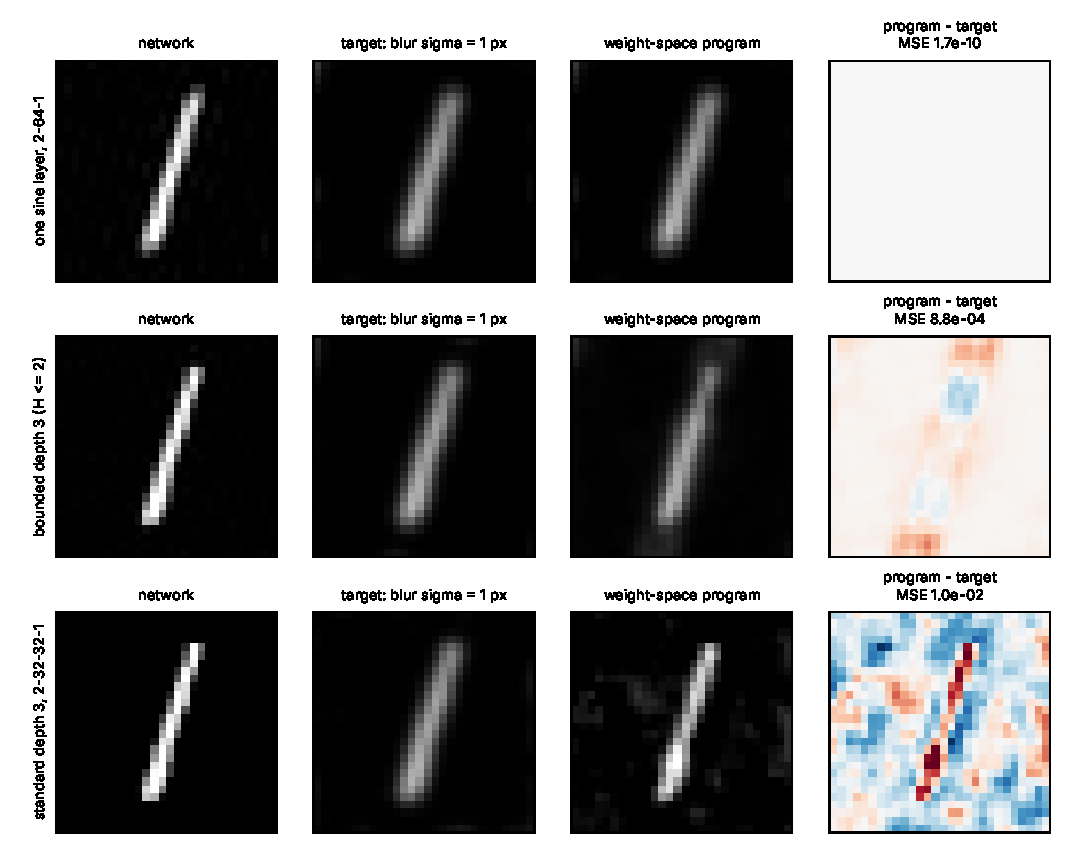
\includegraphics[width=\textwidth]{figures/fig_qualitative.pdf}
\caption{Blur as a weight edit on one image. Top: one sine layer, exact. Middle: depth 3 trained with the harmonic index bounded at 2 (Section~\ref{sec:editable}), the first-order program removes most of the error. Bottom: standard depth 3, the same program adds error.}
\label{fig:qual}
\end{figure}

\section{The price of programmability}
\label{sec:price}
Could one simply use wide one-sine-layer networks? No (Figure~\ref{fig:wd}). At $1{,}025$--$1{,}537$ weights the shallow family reaches $26$--$27$\,dB on MNIST where $2$-$32$-$32$-$1$ ($1{,}185$ weights) reaches $61.5$\,dB; doubling the width from 256 to 1,024 units adds $0.6$\,dB per doubling; a $337$-weight $2$-$16$-$16$-$1$ beats a $4{,}097$-weight $2$-$1024$-$1$. On Fashion-MNIST the matched-parameter gap is $42$\,dB. A least-squares refit of the readout with the trained frequencies held fixed reproduces the trained PSNR exactly, so the dictionary itself is the limit at any time, although it keeps improving slowly with more training (five times the steps add $4.4$\,dB, a prediction we had registered as $<1$\,dB and that failed). For comparison, the best $384$ DCT coefficients of the same images give $34$\,dB. The compression that depth buys comes from composition, i.e.\ from the harmonics that break per-unit programmability.

\begin{figure}[t]\centering
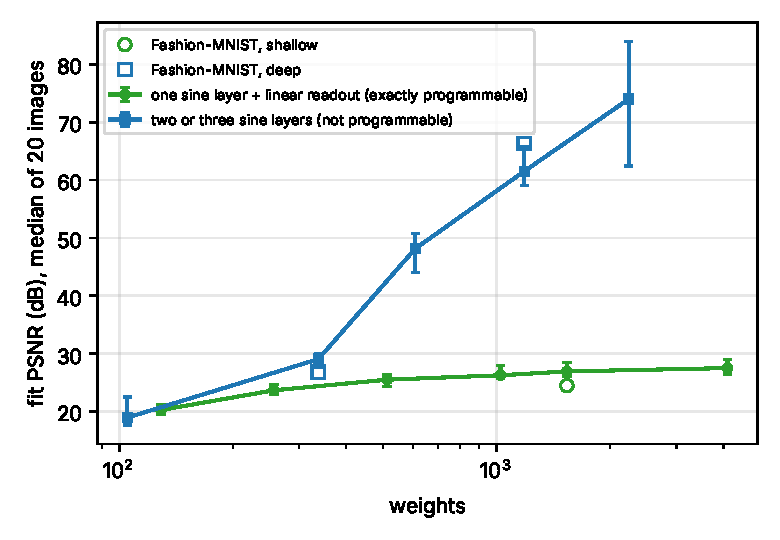
\includegraphics[width=0.6\textwidth]{figures/fig_width_depth.pdf}
\caption{Fit quality against parameter count. Filled: MNIST, median of 20 images with bootstrap intervals; hollow: Fashion-MNIST.}
\label{fig:wd}
\end{figure}

\section{Buying programmability back}
\label{sec:editable}
If the failure is governed by $H_j$, training can control it. We project after every Adam step so that every hidden unit satisfies $\sum_i|a_{ij}|\le B$ (no unit is switched off). Table~\ref{tab:editable} shows a monotone, seed-stable trade-off on both datasets: as $B$ grows from 1 to 8 the fit rises from $22$ to $68$\,dB and the first-order blur program degrades from $0.03\times$ to about $1\times$ the no-edit error on MNIST, and to $2.3$--$2.9\times$ on Fashion-MNIST. At matched $H$ the projection dominates an $L_1$ penalty on the same weights ($B=2$: $28.8$\,dB and $0.15$; penalty: $27.7$\,dB and $0.40$), whose apparent gains came from pruning units. The useful operating point is dataset dependent: $B=4$ removes about $70\%$ of the blur error on digits (at $40$\,dB) but only $50\%$ on clothing textures (at $38$\,dB), a registered prediction that failed; $B=2$ behaves the same on both datasets ($29$ and $27$\,dB, $85\%$ removed).

\begin{table}[t]\centering\small
\caption{Swing-bound training, $2$-$32$-$32$-$1$: fit PSNR and first-order blur program error / no-edit error (function space), two seeds.}
\label{tab:editable}
\begin{tabular}{lcccc}\toprule
bound $B$ & MNIST PSNR & MNIST blur ratio & Fashion PSNR & Fashion blur ratio\\\midrule
1 & 22.1 / 22.8 & 0.025 / 0.035 & 21.2 / 21.8 & 0.042 / 0.032\\
2 & 28.8 / 28.8 & 0.150 / 0.161 & 26.4 / 26.8 & 0.202 / 0.176\\
4 & 39.7 / 40.5 & 0.280 / 0.252 & 38.3 / 37.2 & 0.483 / 0.523\\
8 & 67.8 / 68.7 & 1.09 / 0.77 & 61.3 / 68.0 & 2.95 / 2.30\\
standard & 61.5 & 1.63 & 66.3 & --\\\bottomrule
\end{tabular}
\end{table}

\section{Related work}
Weight-space learning studies networks as inputs: permutation-equivariant functionals~\citep{zhou2023nfn,zhou2023nft}, graph metanetworks~\citep{kofinas2025internal}, INR zoos~\citep{ma2024implicitzoo}, and a recent survey~\citep{han2026survey}. The NFN editing tasks (dilate, contrast) are learned maps from INR weights to INR weights; our Section~\ref{sec:algebra} gives the closed form for the contrast task and Section~\ref{sec:depth} a bound on what any readout-only editor can do for dilation. The structured-dictionary view of INRs~\citep{yuce2022structured} supplies the harmonic expansion behind Section~\ref{sec:depth}; spectral bias in coordinate networks~\citep{tancik2020fourier} is why the shallow family fits poorly. Croppable INRs~\citep{ashkenazi2024croppable} edit weights for one operation by construction. Weight-space programming~\citep{takehi2026sparks} and weight oracles~\citep{kabra2026oracles} ask whether a language model can read or write weights; we characterise the object those studies would act on. In arbitrary-scale super-resolution, decoders with a local Fourier field and a linear readout make the pixel-footprint integral exact~\citep{lee2022lte}; that architecture is the one-sine-layer case of our algebra with the capacity moved into an encoder.

\section{Discussion}
\paragraph{Where programmability is cheap.} For a standalone image INR it costs 35--42\,dB at matched parameters. The setting where it should cost little is a conditional INR whose encoder carries the capacity and whose decoder is a sinusoidal dictionary with a linear readout, as in arbitrary-scale super-resolution; there anti-aliased resampling, footprint integration and derivative features are weight edits. We state this as the prediction for the next study, not a result of this one.
\paragraph{Can a model discover these programs?} In a registered pilot, a frontier model given only the weights and one reply reproduced every coordinate- and readout-layer program exactly, including a four-pixel shift that required 32 phase updates, but read the stored digit at chance (1 of 5) and, asked to dilate, reached for a global output gain. Reading and non-local editing require code over the weights; measuring that is future work.
\paragraph{Limitations.} Grey-scale $28\times28$ images, SIRENs only, one training recipe; harmonic index and swing bound are specific to sinusoidal layers; pixel-space targets understate the exactness of function-space programs and should not be used alone.

\paragraph{Reproducibility.} Code, frozen protocols, prediction ledgers, zoo indices and per-network results are released; \texttt{scripts/reproduce.sh} rebuilds every number on CPU in about six hours.

\bibliographystyle{plainnat}
\bibliography{refs}

\appendix
\section{Prediction ledger}
\label{app:ledger}
Every stage froze its predictions before running. Outcomes: Stage 02 (programs by layer and depth), Q1 shallow blur $<2\times10^{-4}$ against the pixel-space target: failed as written (max $9.6\times10^{-4}$), exact against the function-space target ($7\times10^{-10}$ max); Q2 rms attenuation partially blurs deep networks: failed in the worse direction (ratio 2.1); Q3 network-level correlation with the harmonic index: failed ($\rho=-0.04$, no range), unit-level $\rho=0.85$; Q4 readout cannot do morphology: half failed, the erosion half a target-energy artefact ($R^2=0.37$); Q5 contrast by the readout $<10^{-6}$: passed. Stage 03 (width vs depth): W1 gap $>25$\,dB passed (35); W2 saturation passed (0.6\,dB per doubling); W3 ten thousand steps $<1$\,dB: failed ($+4.4$); W4 small deep beats large shallow passed; W5 programmability unchanged passed. Stage 04 v2 (editable training): E1 monotone passed (4/4 series); E2 datasets within factor 2: failed at $B=8$ (2.8); E3 projection dominates penalty passed (both seeds); E4 $B=4$ operating point: failed on Fashion-MNIST (ratio 0.50); E5 passed.
\end{document}
